\section{Скриншоты приложения}

Приложение оптимизированно для разных разрешений экрана (больше 900, 700, 480 пиксей по ширине) а так же версия для печати. Для этого использовались @media-правила, встроенные в CSS.

Приложение протестировано в браузере Google Chrome на следующих операционных системах:
\begin{itemize}
	\item Windows 7 x64, версия 43.0.2357.81
	\item Mac OS X, версия 43.0.2357.81
	\item Android 4.4.4, версия 43.0.2357.92
	\item iOS 8.3, версия 42.0.2311.47
\end{itemize} 

\begin{figure}[H]
	\centering
	\begin{subfigure}[t]{0.9\textwidth}
		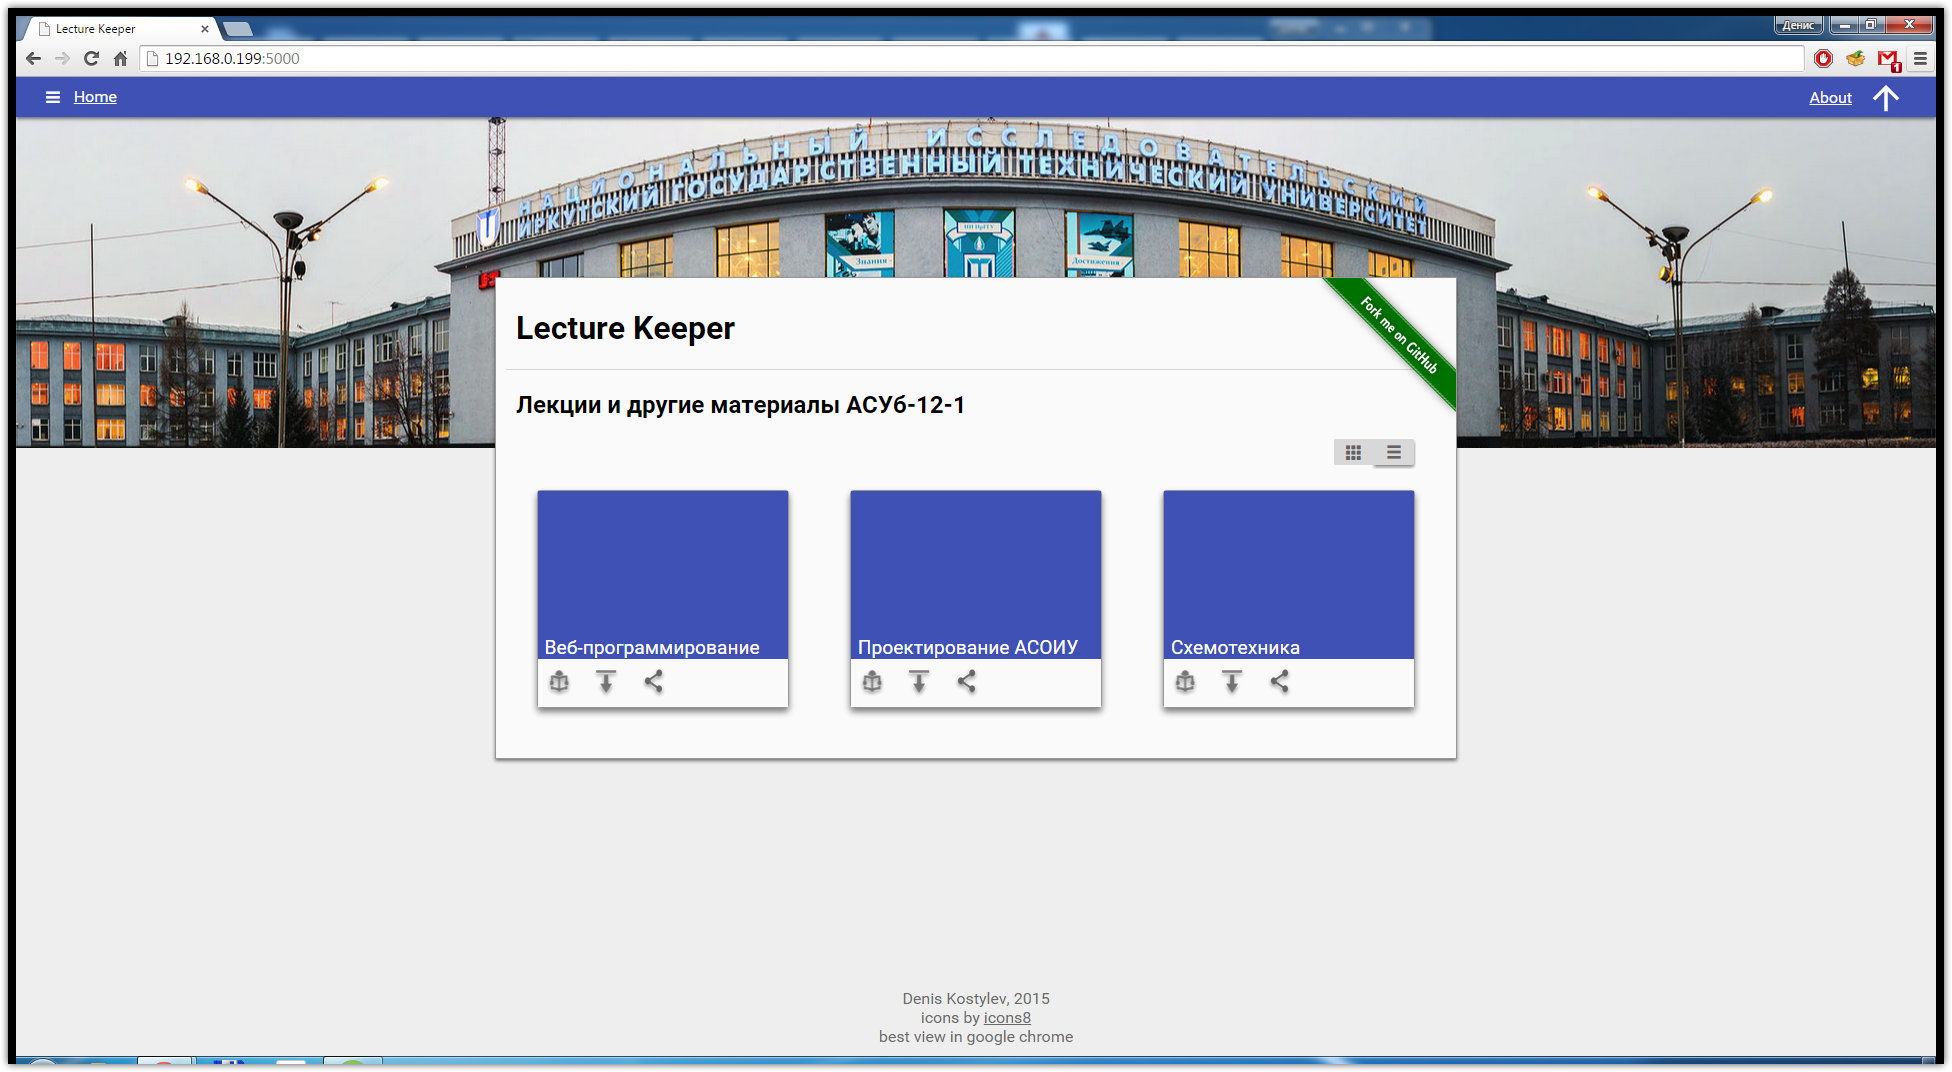
\includegraphics[width=\textwidth]{pics/screens/win7_1000_index_card.png}
		\caption{Windows 7}
	\end{subfigure}
	\begin{subfigure}[b]{0.4\textwidth}
		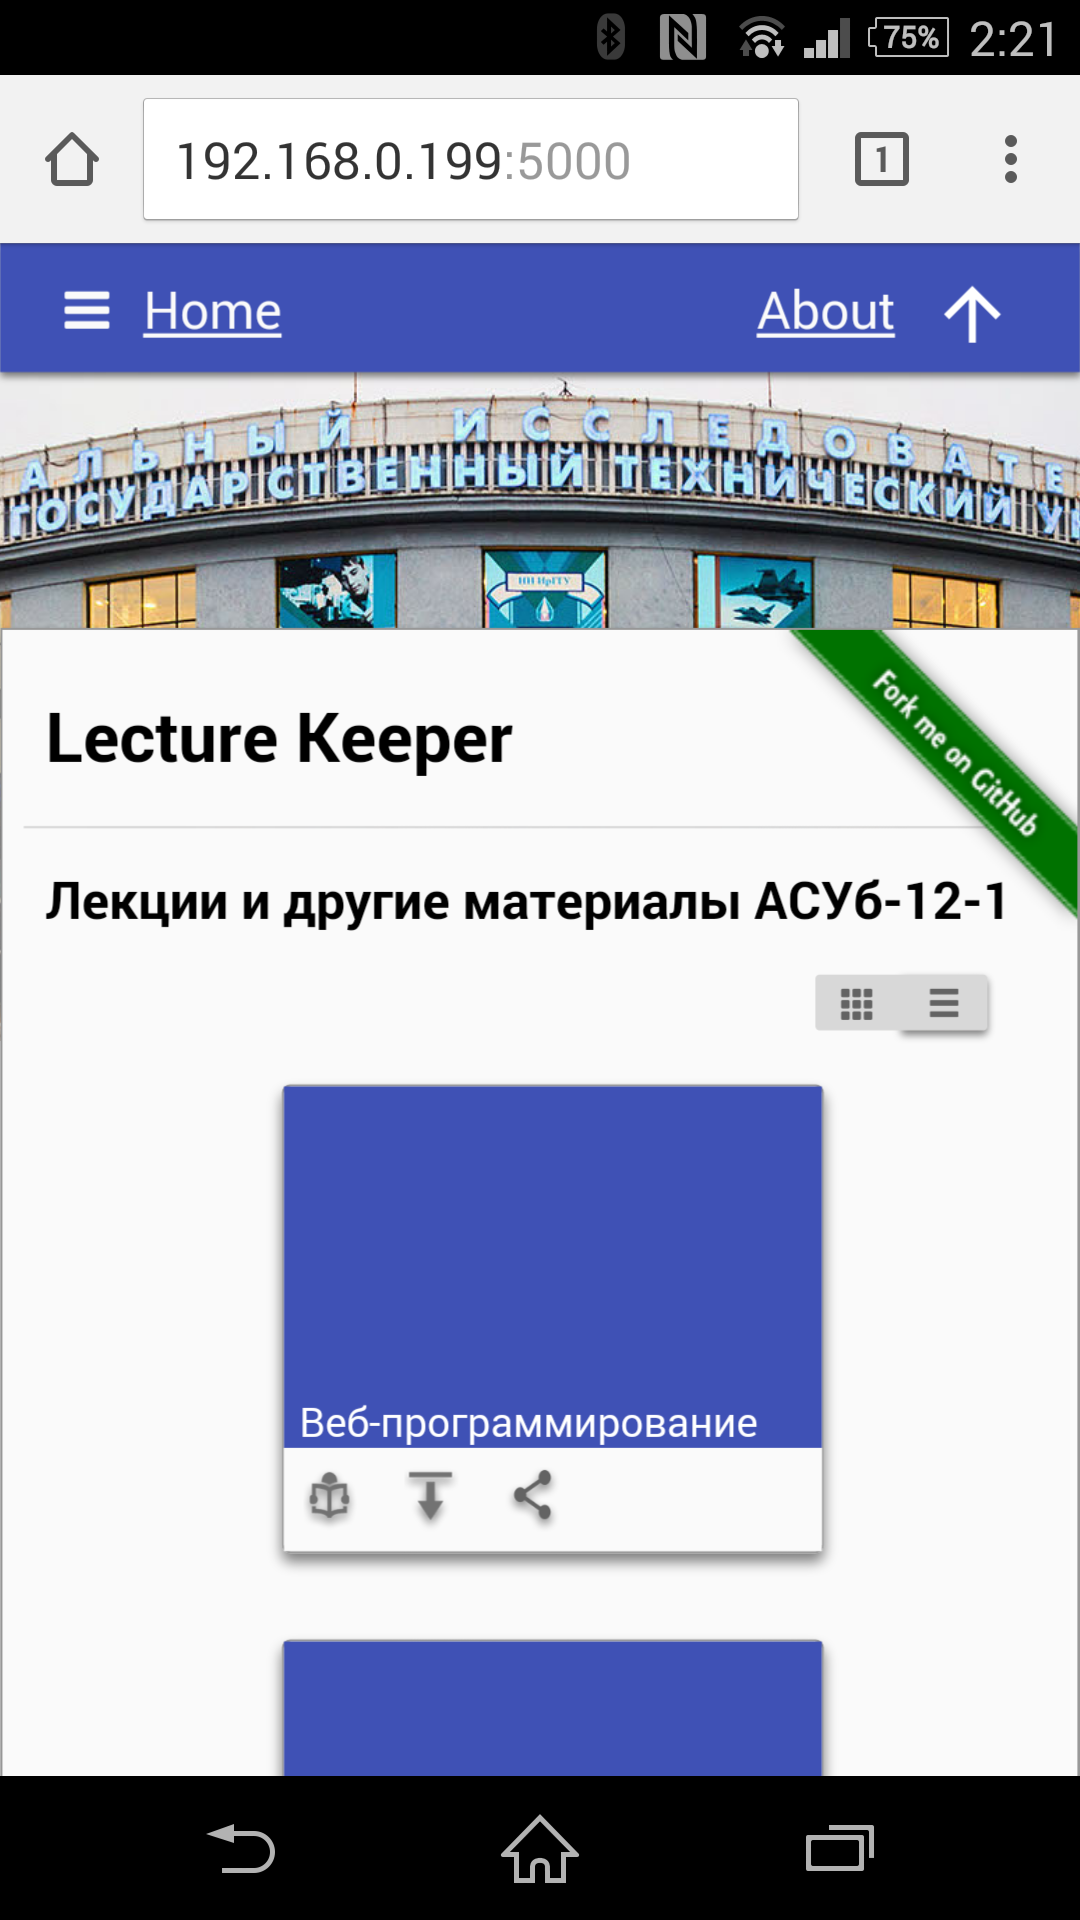
\includegraphics[width=\textwidth]{pics/screens/android_index_card.png}
		\caption{Android}
	\end{subfigure}
	\quad
	\begin{subfigure}[b]{0.4\textwidth}
		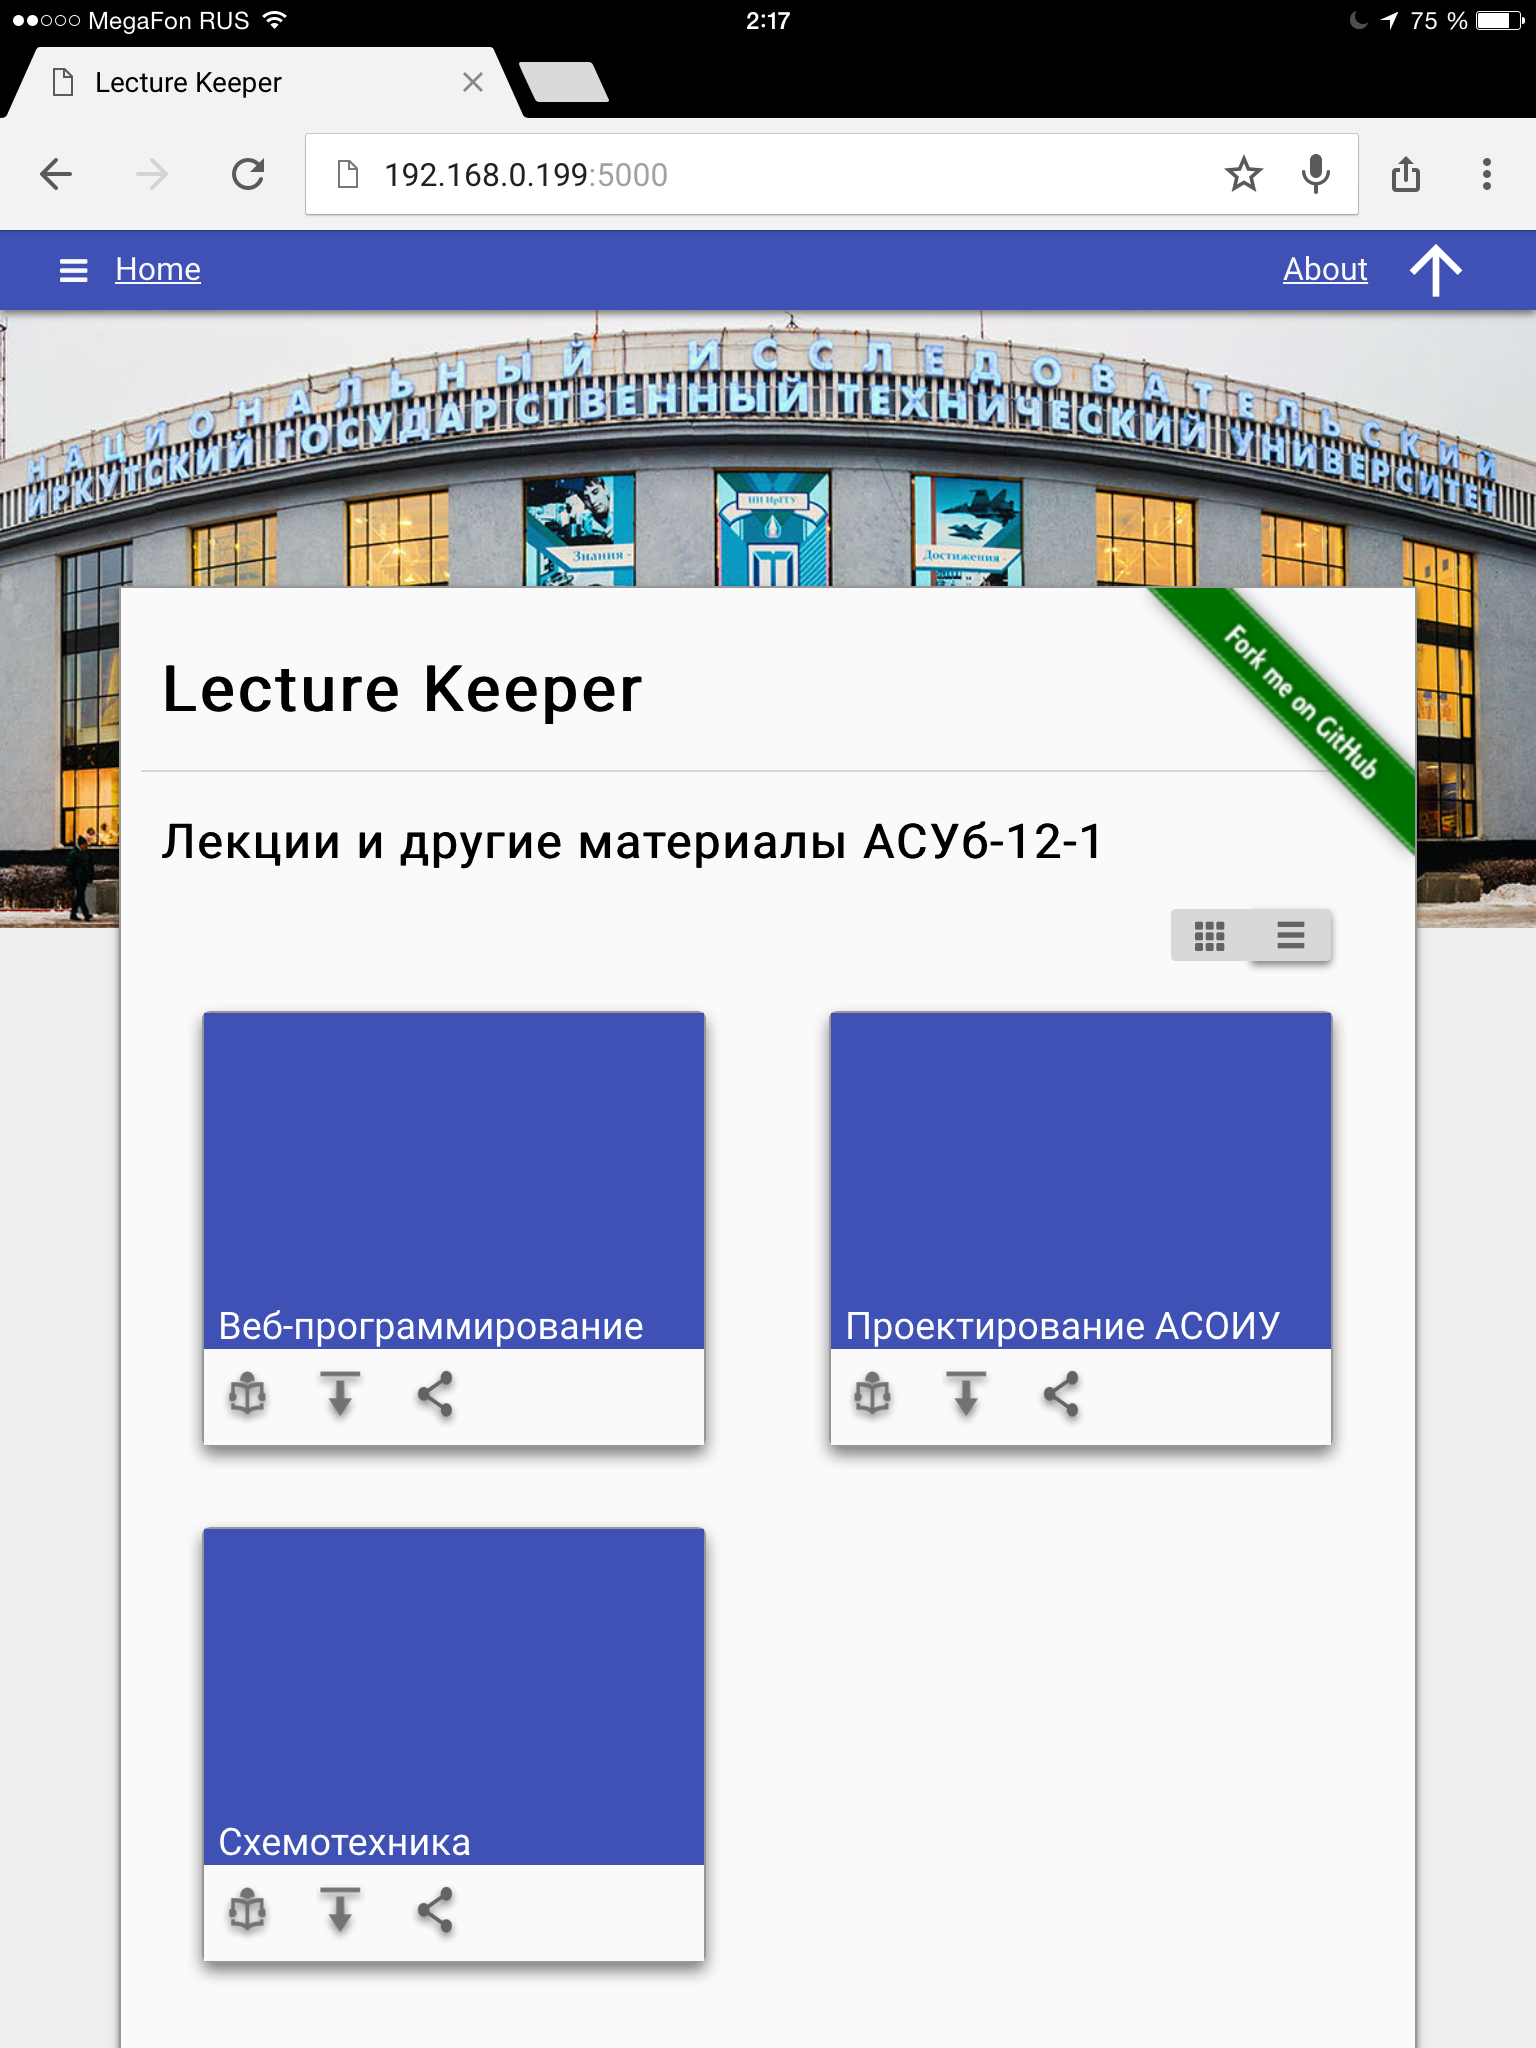
\includegraphics[width=\textwidth]{pics/screens/ipad_index_card.png}
		\caption{iOS}
	\end{subfigure}
	\caption{Главная страница с дисциплинами в виде карточек}
\end{figure}

\begin{figure}[H]
	\centering
	\begin{subfigure}[r]{0.4\textwidth}
		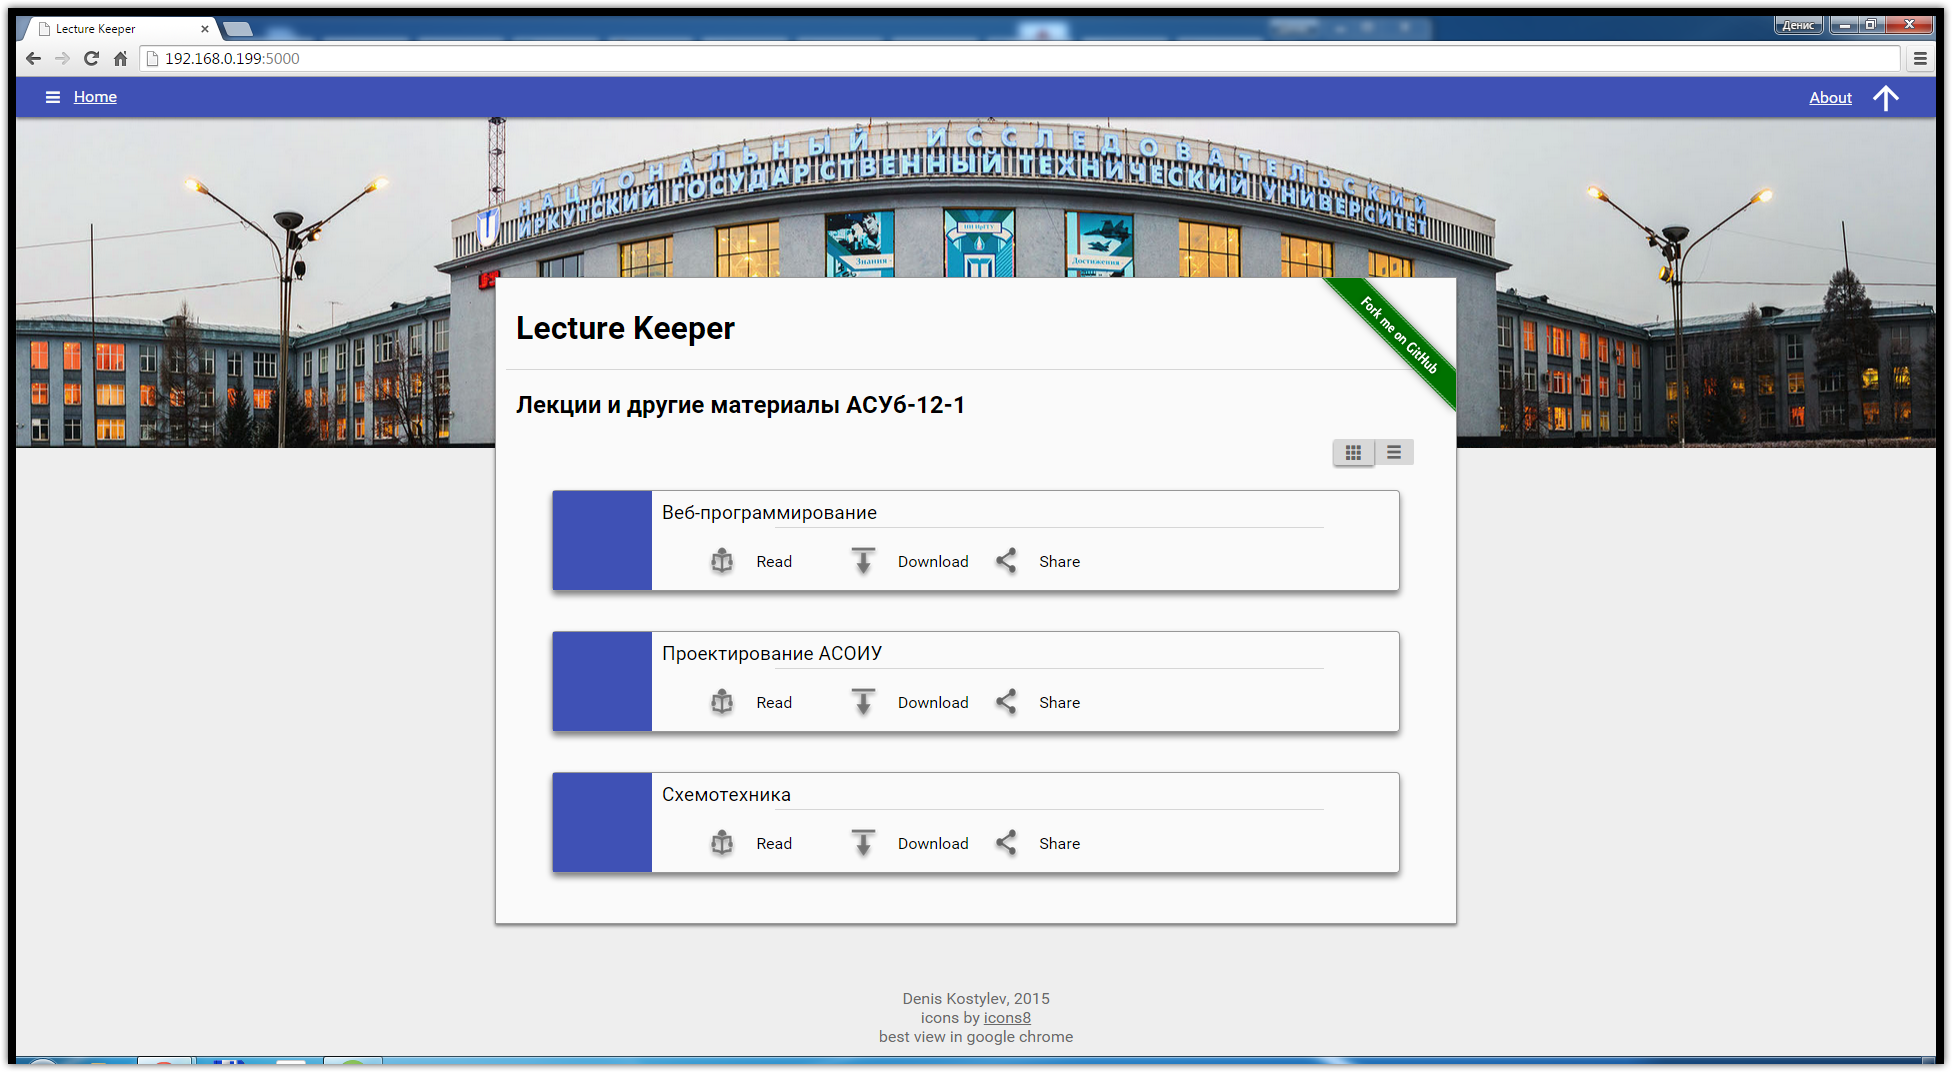
\includegraphics[width=\textwidth]{pics/screens/win7_1000_index_list.png}
		\caption{Windows 7}
	\end{subfigure}
	\quad
	\begin{subfigure}[l]{0.4\textwidth}
		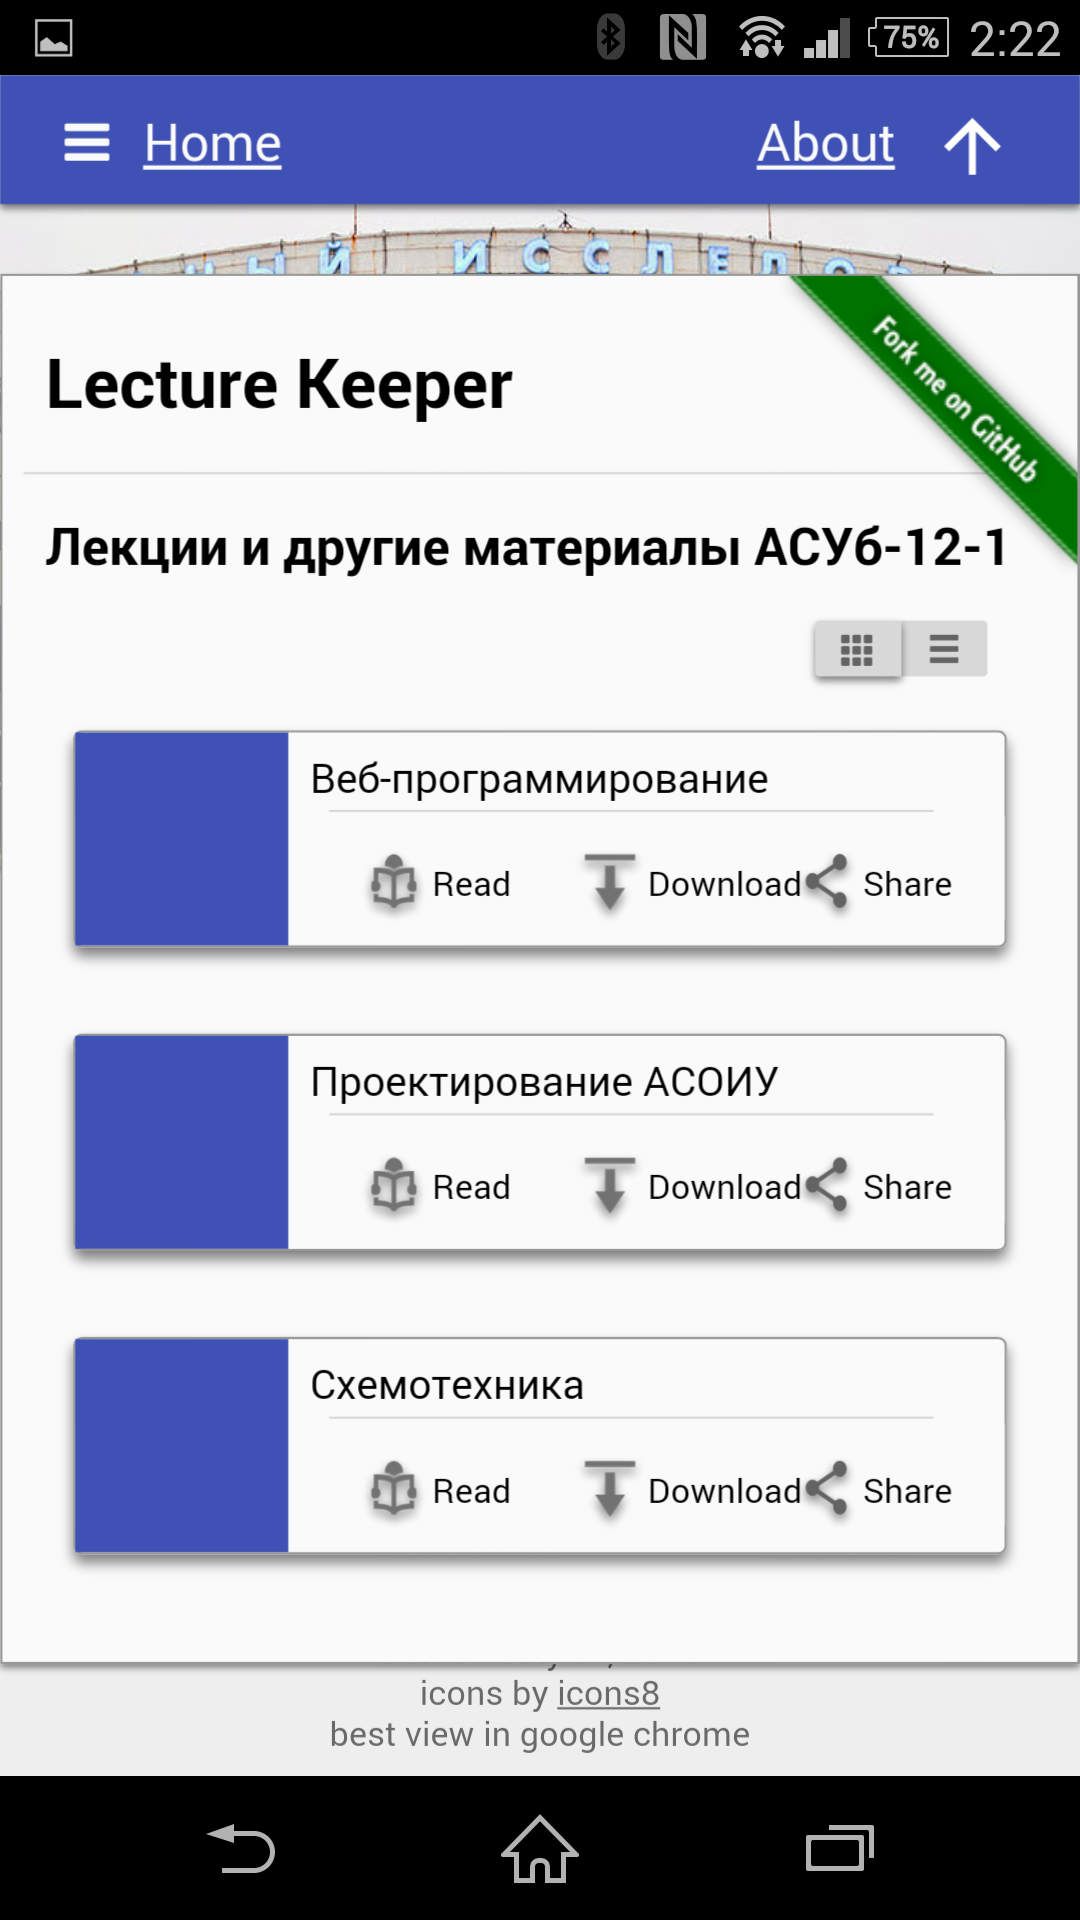
\includegraphics[width=\textwidth]{pics/screens/android_index_list.png}
		\caption{Android}
	\end{subfigure}
	\caption{Главная страница с дисциплинами в виде списка}
\end{figure}

\begin{figure}[H]
	\centering
	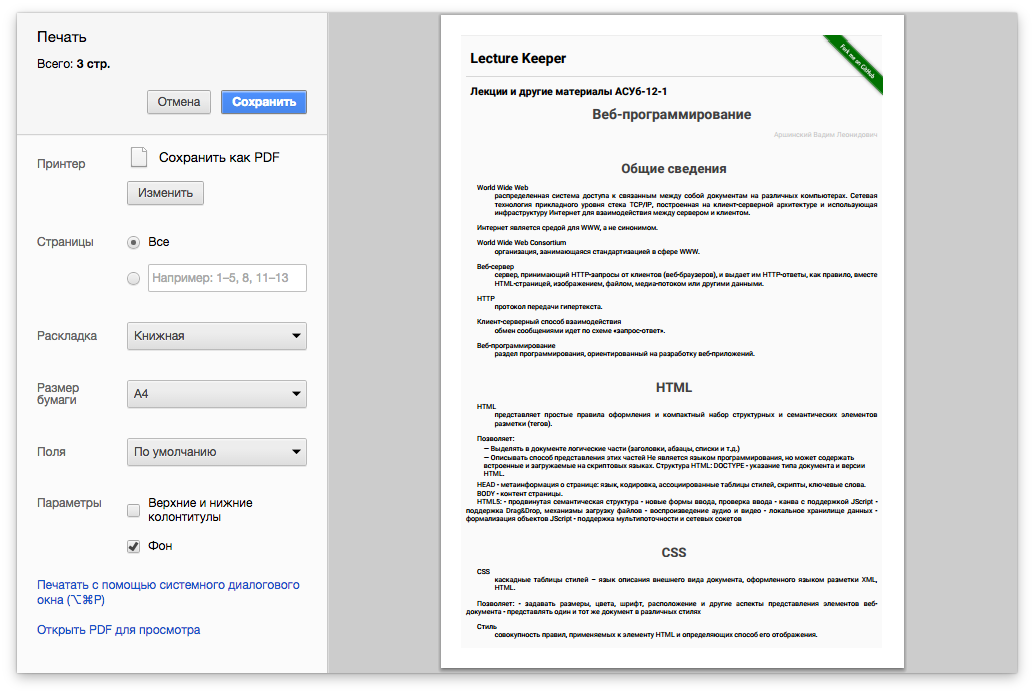
\includegraphics[width=0.7\textwidth]{pics/screens/print.png}
	\caption{Версия для печати}
\end{figure}

\begin{figure}[H]
	\centering
	\begin{subfigure}[t]{0.9\textwidth}
		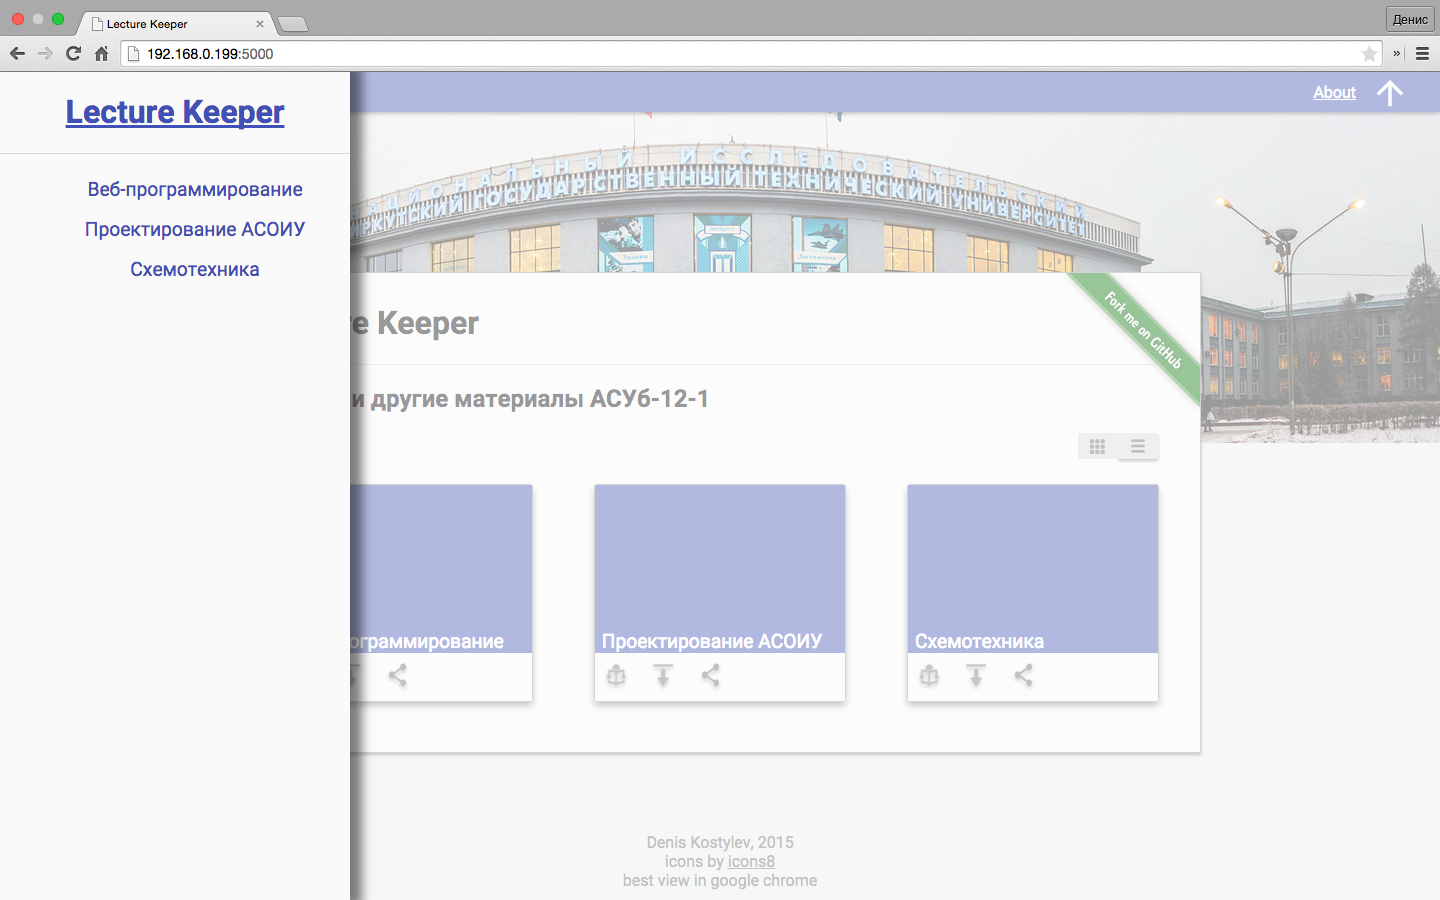
\includegraphics[width=\textwidth]{pics/screens/mac_1000_menu.png}
		\caption{Mac OS X}
	\end{subfigure}
	\begin{subfigure}[b]{0.4\textwidth}
		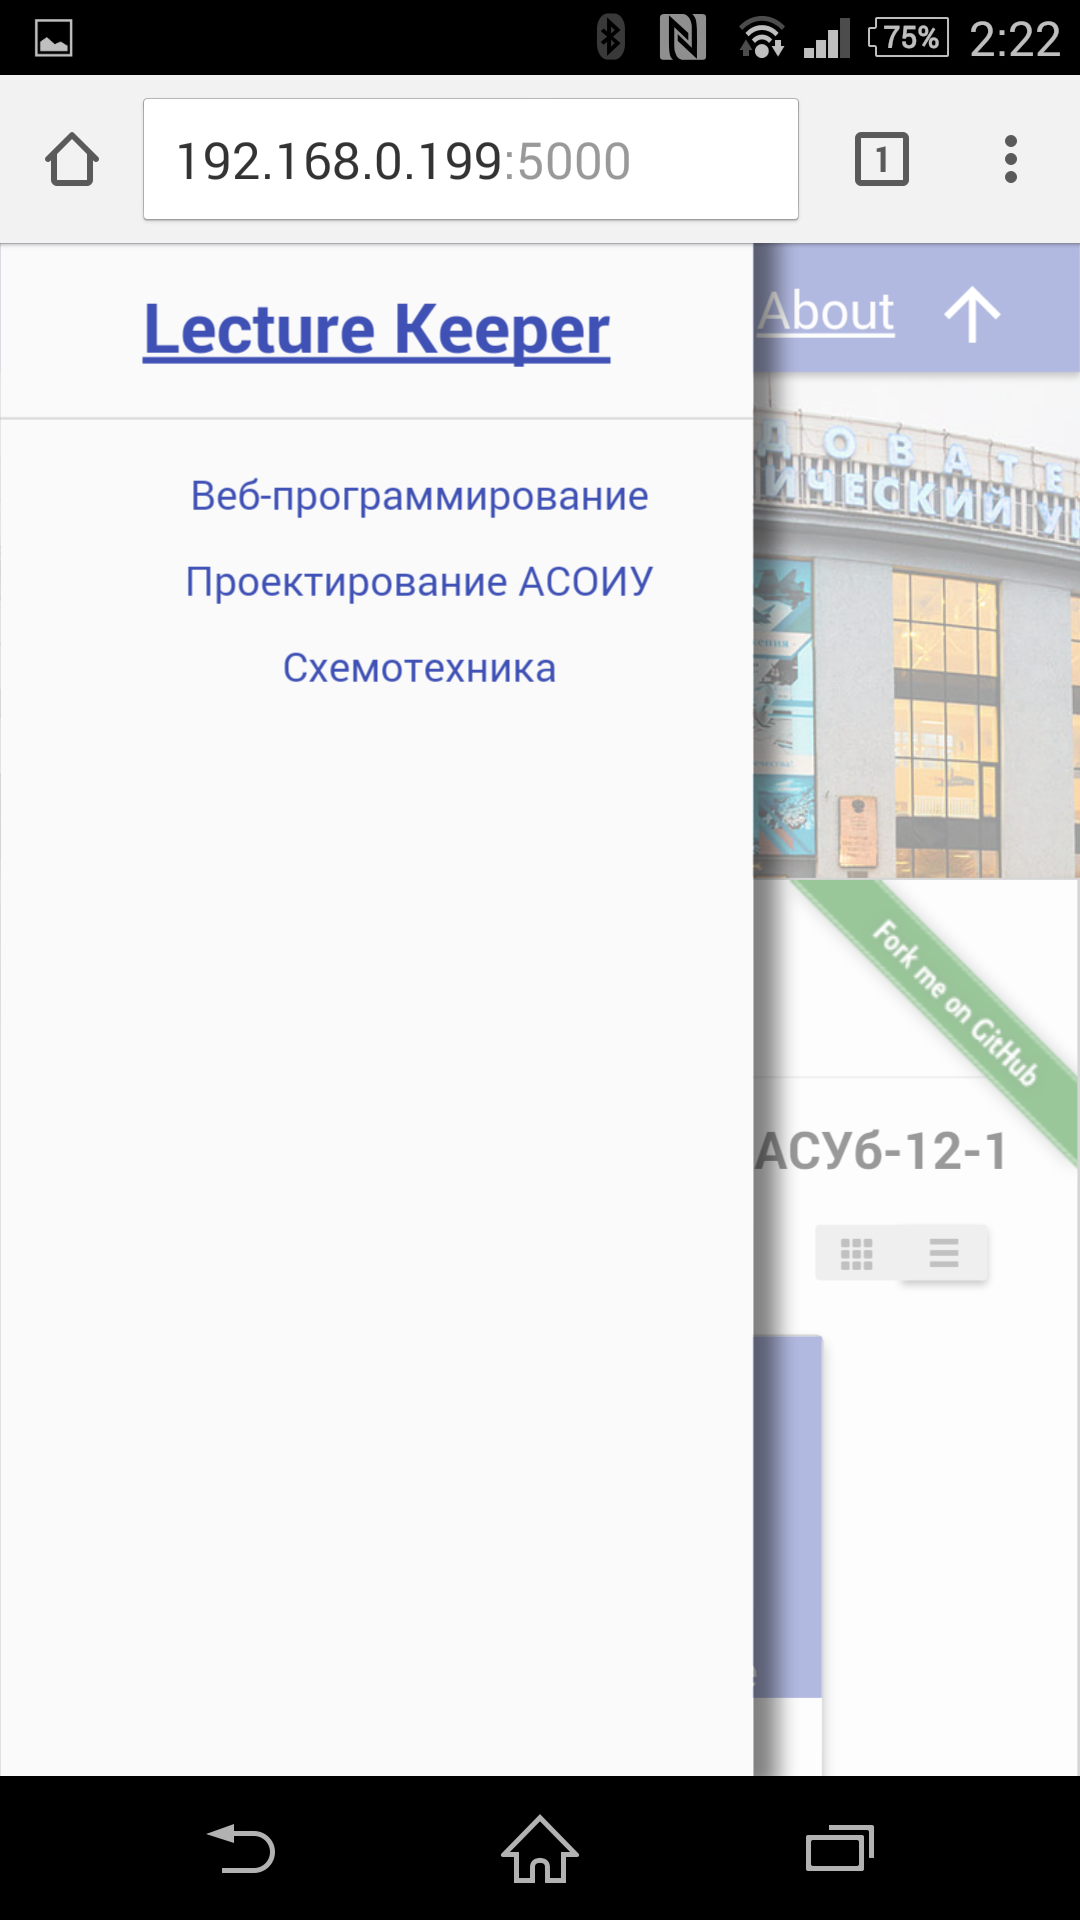
\includegraphics[width=\textwidth]{pics/screens/android_menu.png}
		\caption{Android}
	\end{subfigure}
	\begin{subfigure}[b]{0.4\textwidth}
		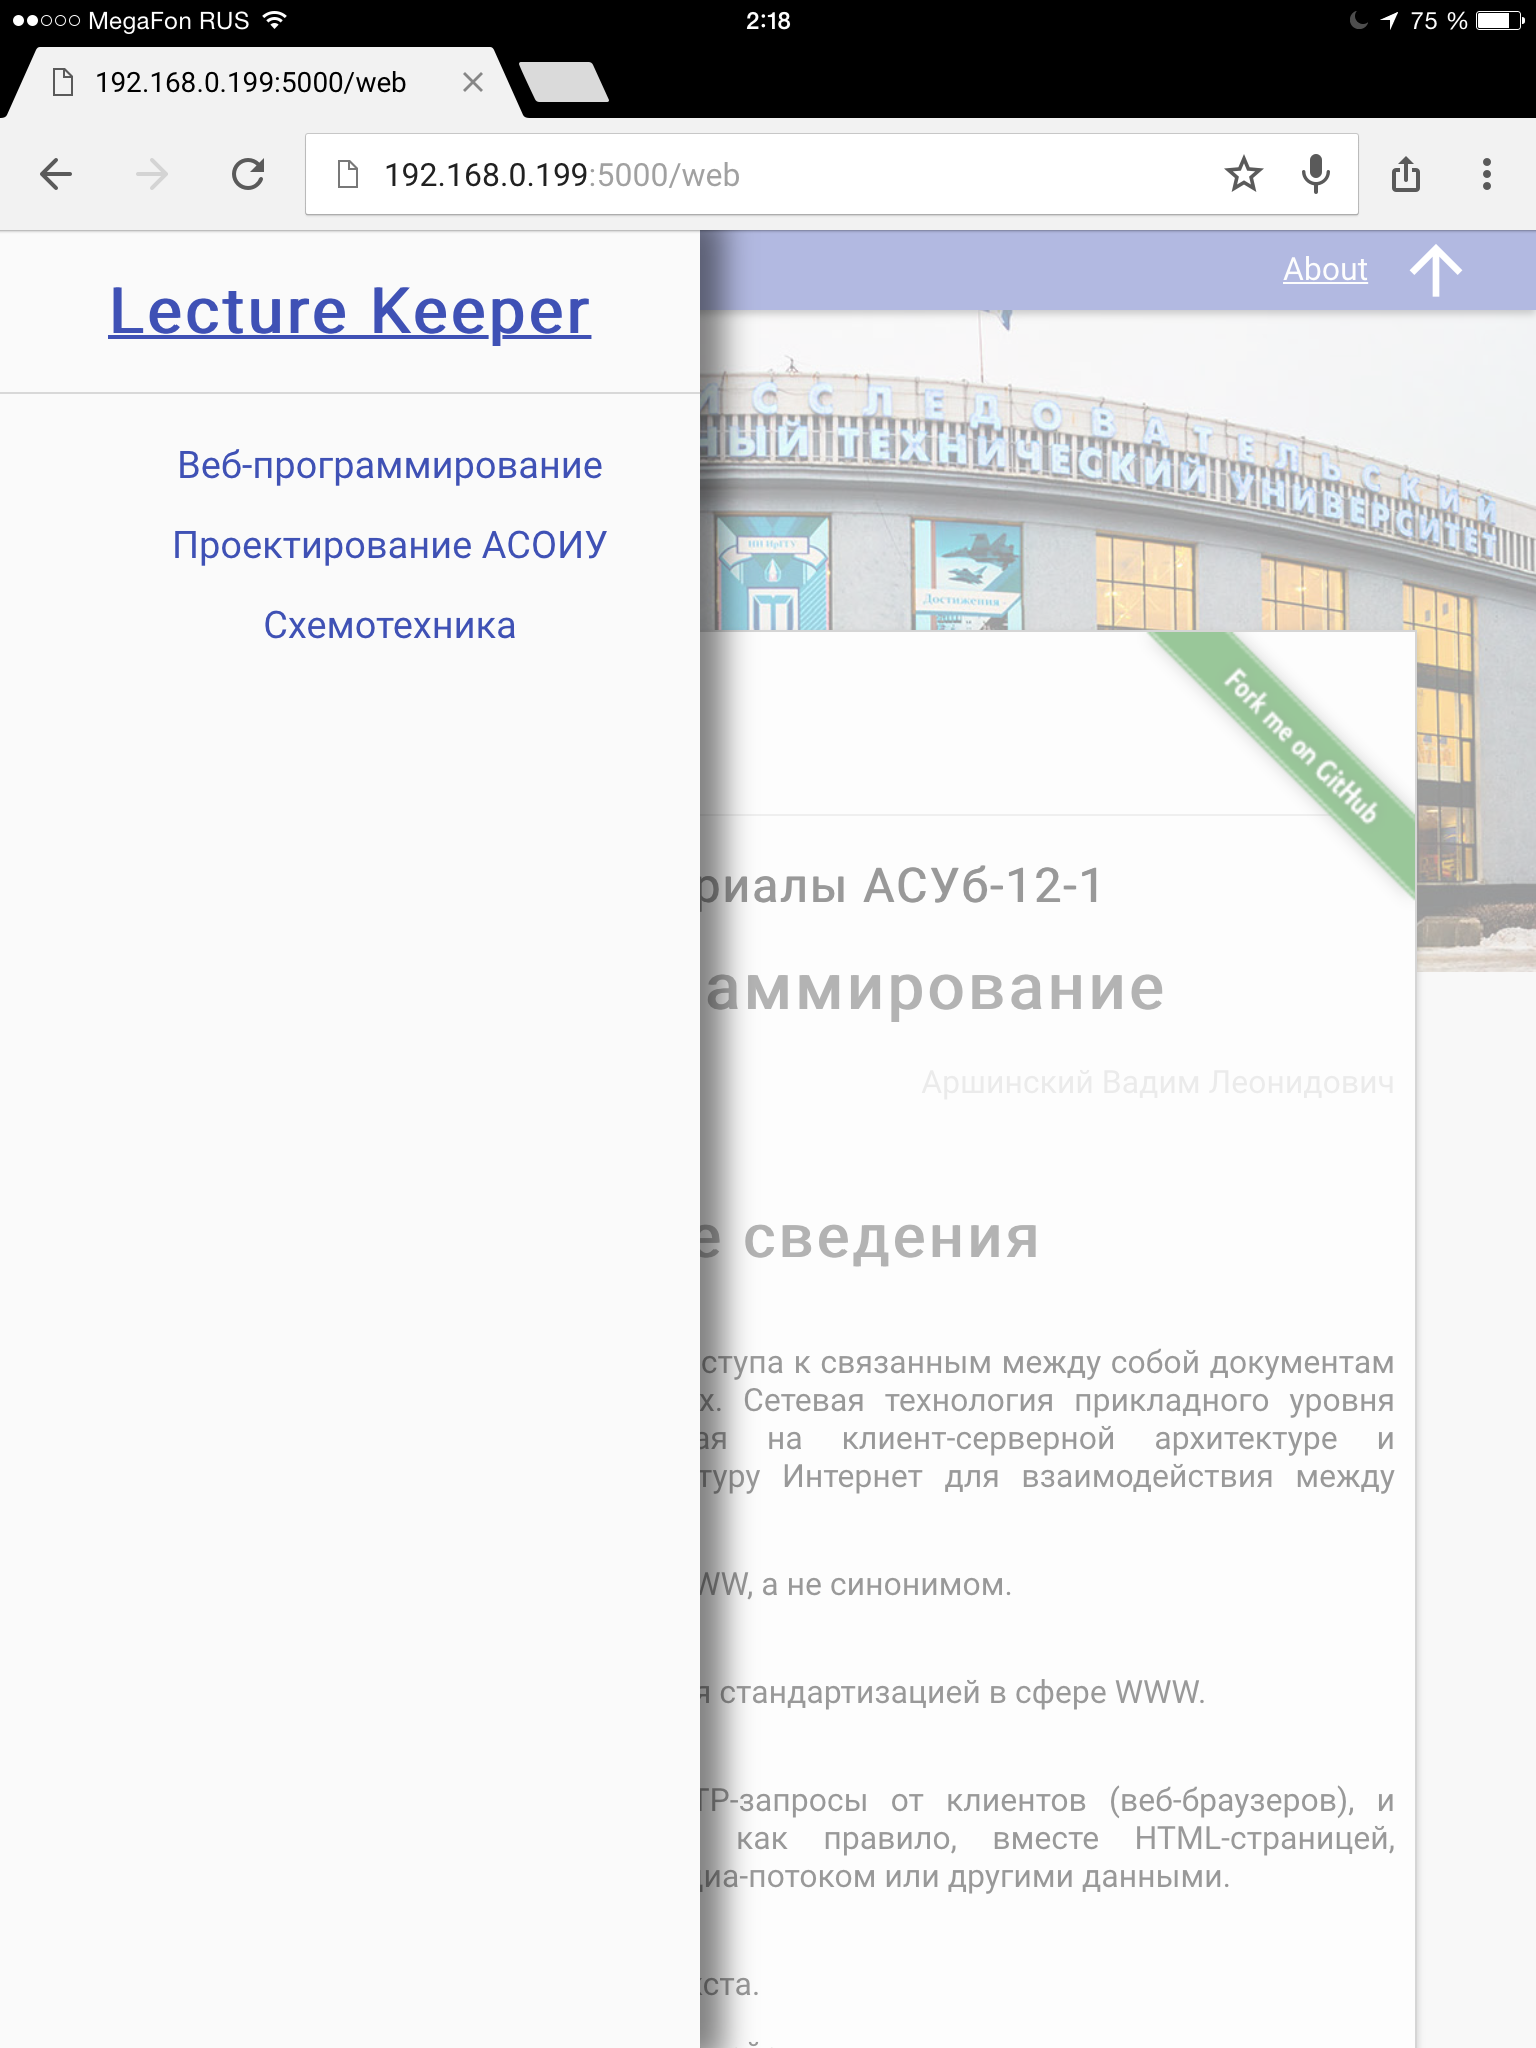
\includegraphics[width=\textwidth]{pics/screens/ipad_menu.png}
		\caption{iOS}
	\end{subfigure}
	\caption{Меню с разными разрешениями экранов}
\end{figure}

\begin{figure}[H]
	\centering
	\begin{subfigure}[t]{0.9\textwidth}
		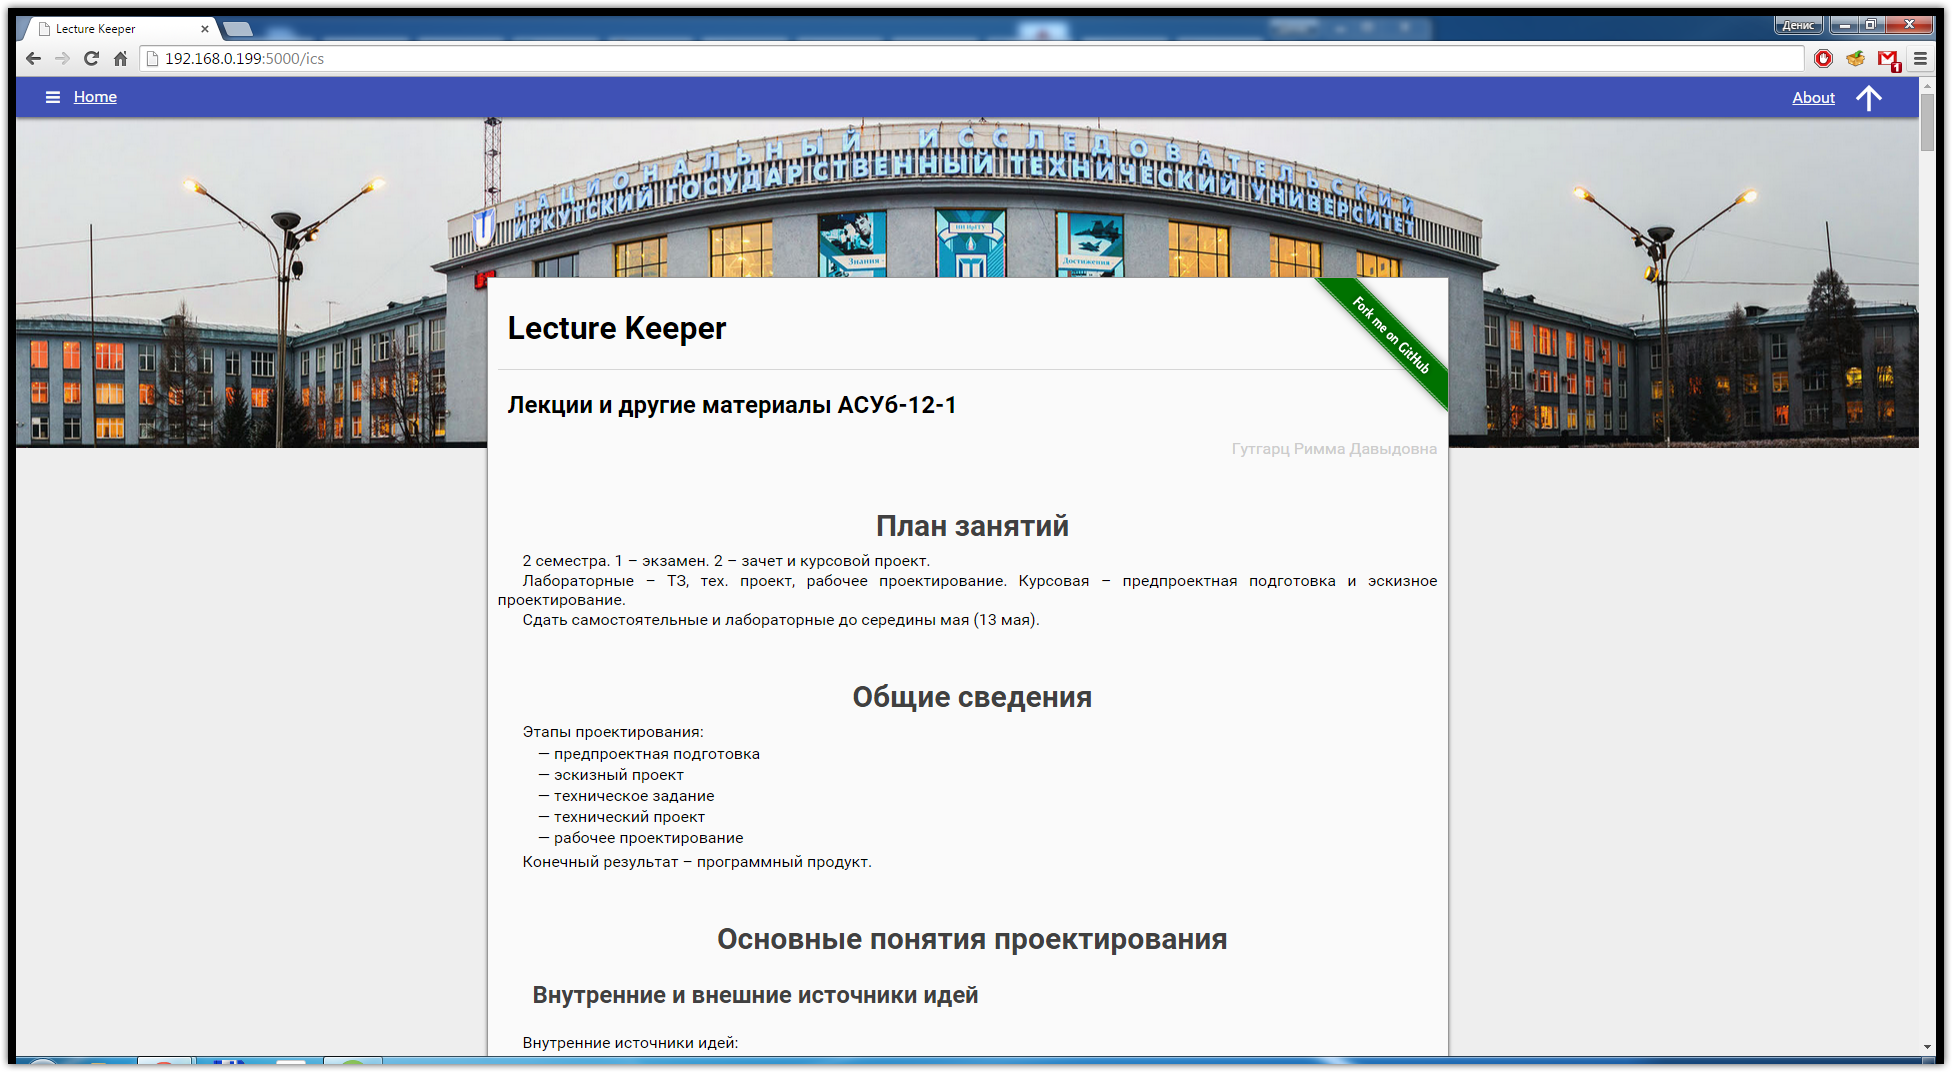
\includegraphics[width=\textwidth]{pics/screens/win7_1000_lec.png}
		\caption{Windows 7}
	\end{subfigure}
	\begin{subfigure}[b]{0.4\textwidth}
		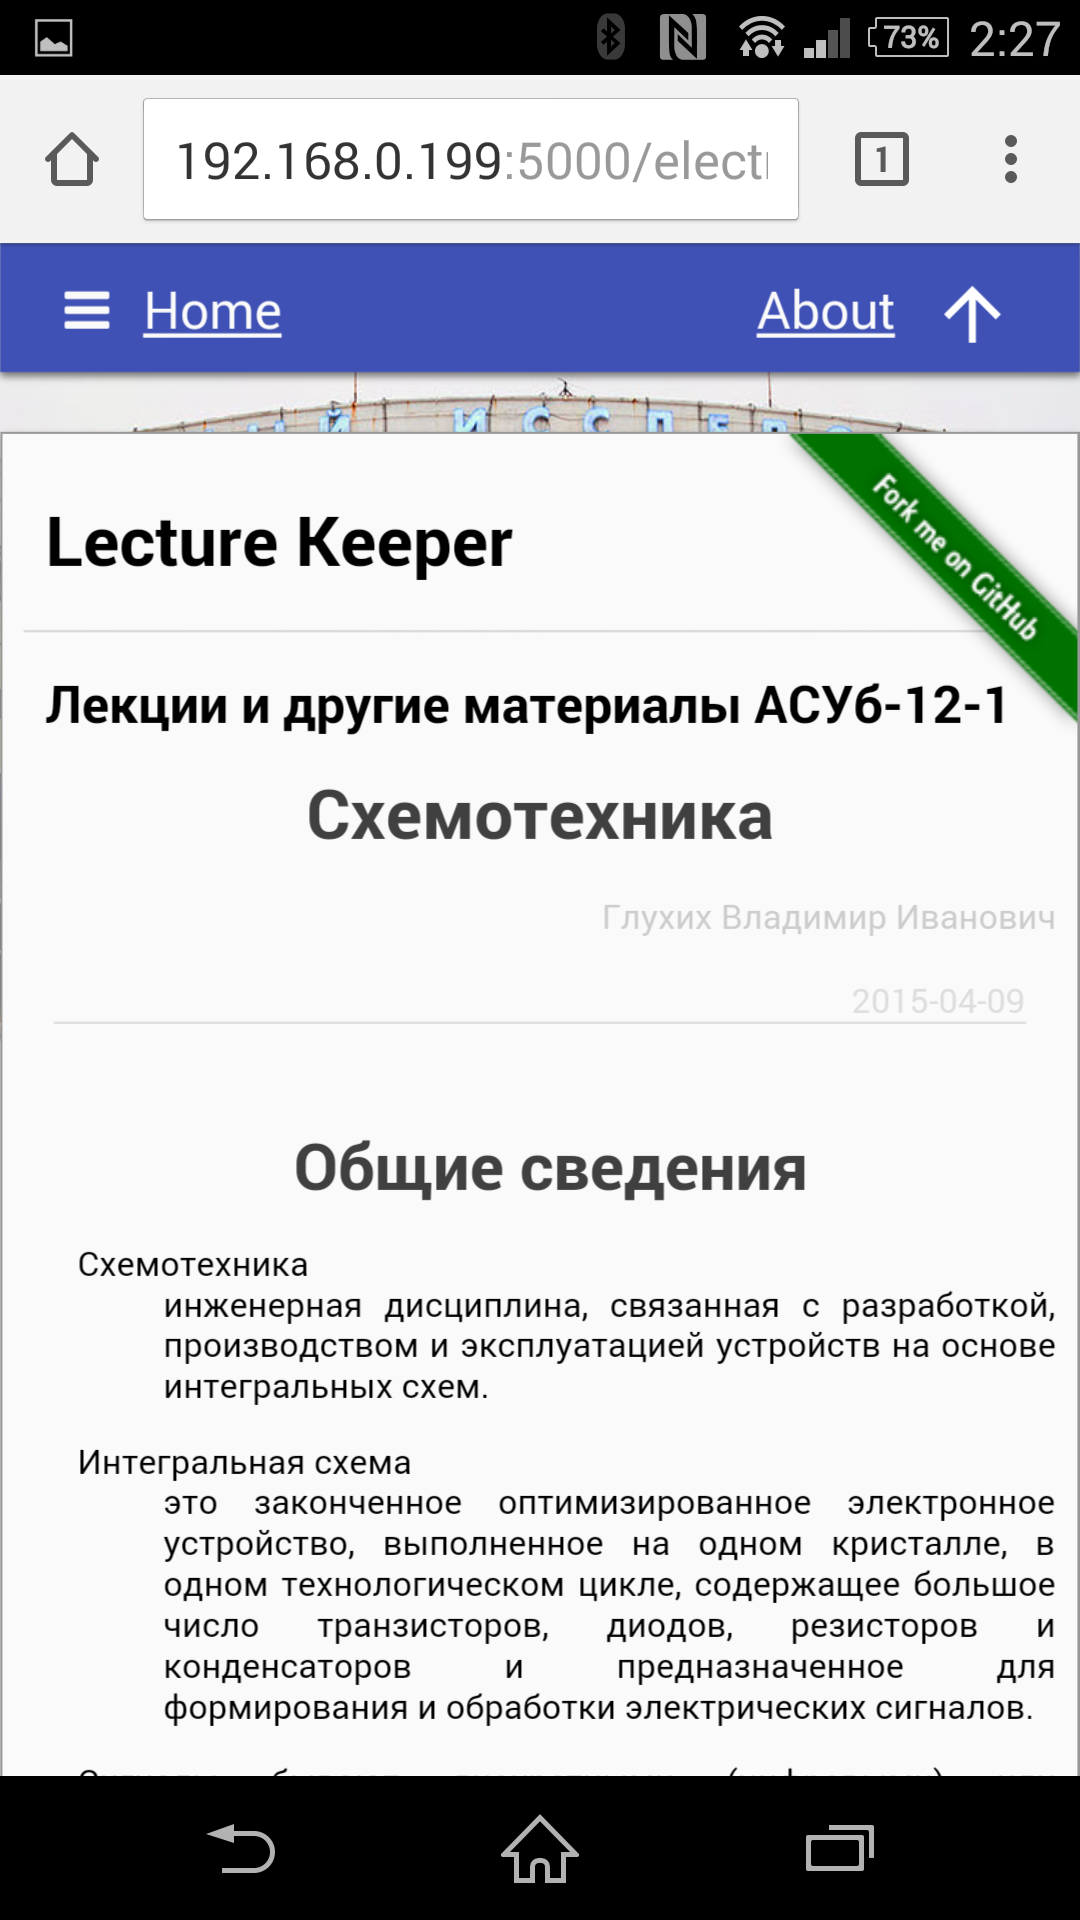
\includegraphics[width=\textwidth]{pics/screens/android_lec.png}
		\caption{Android}
	\end{subfigure}
	\begin{subfigure}[b]{0.4\textwidth}
		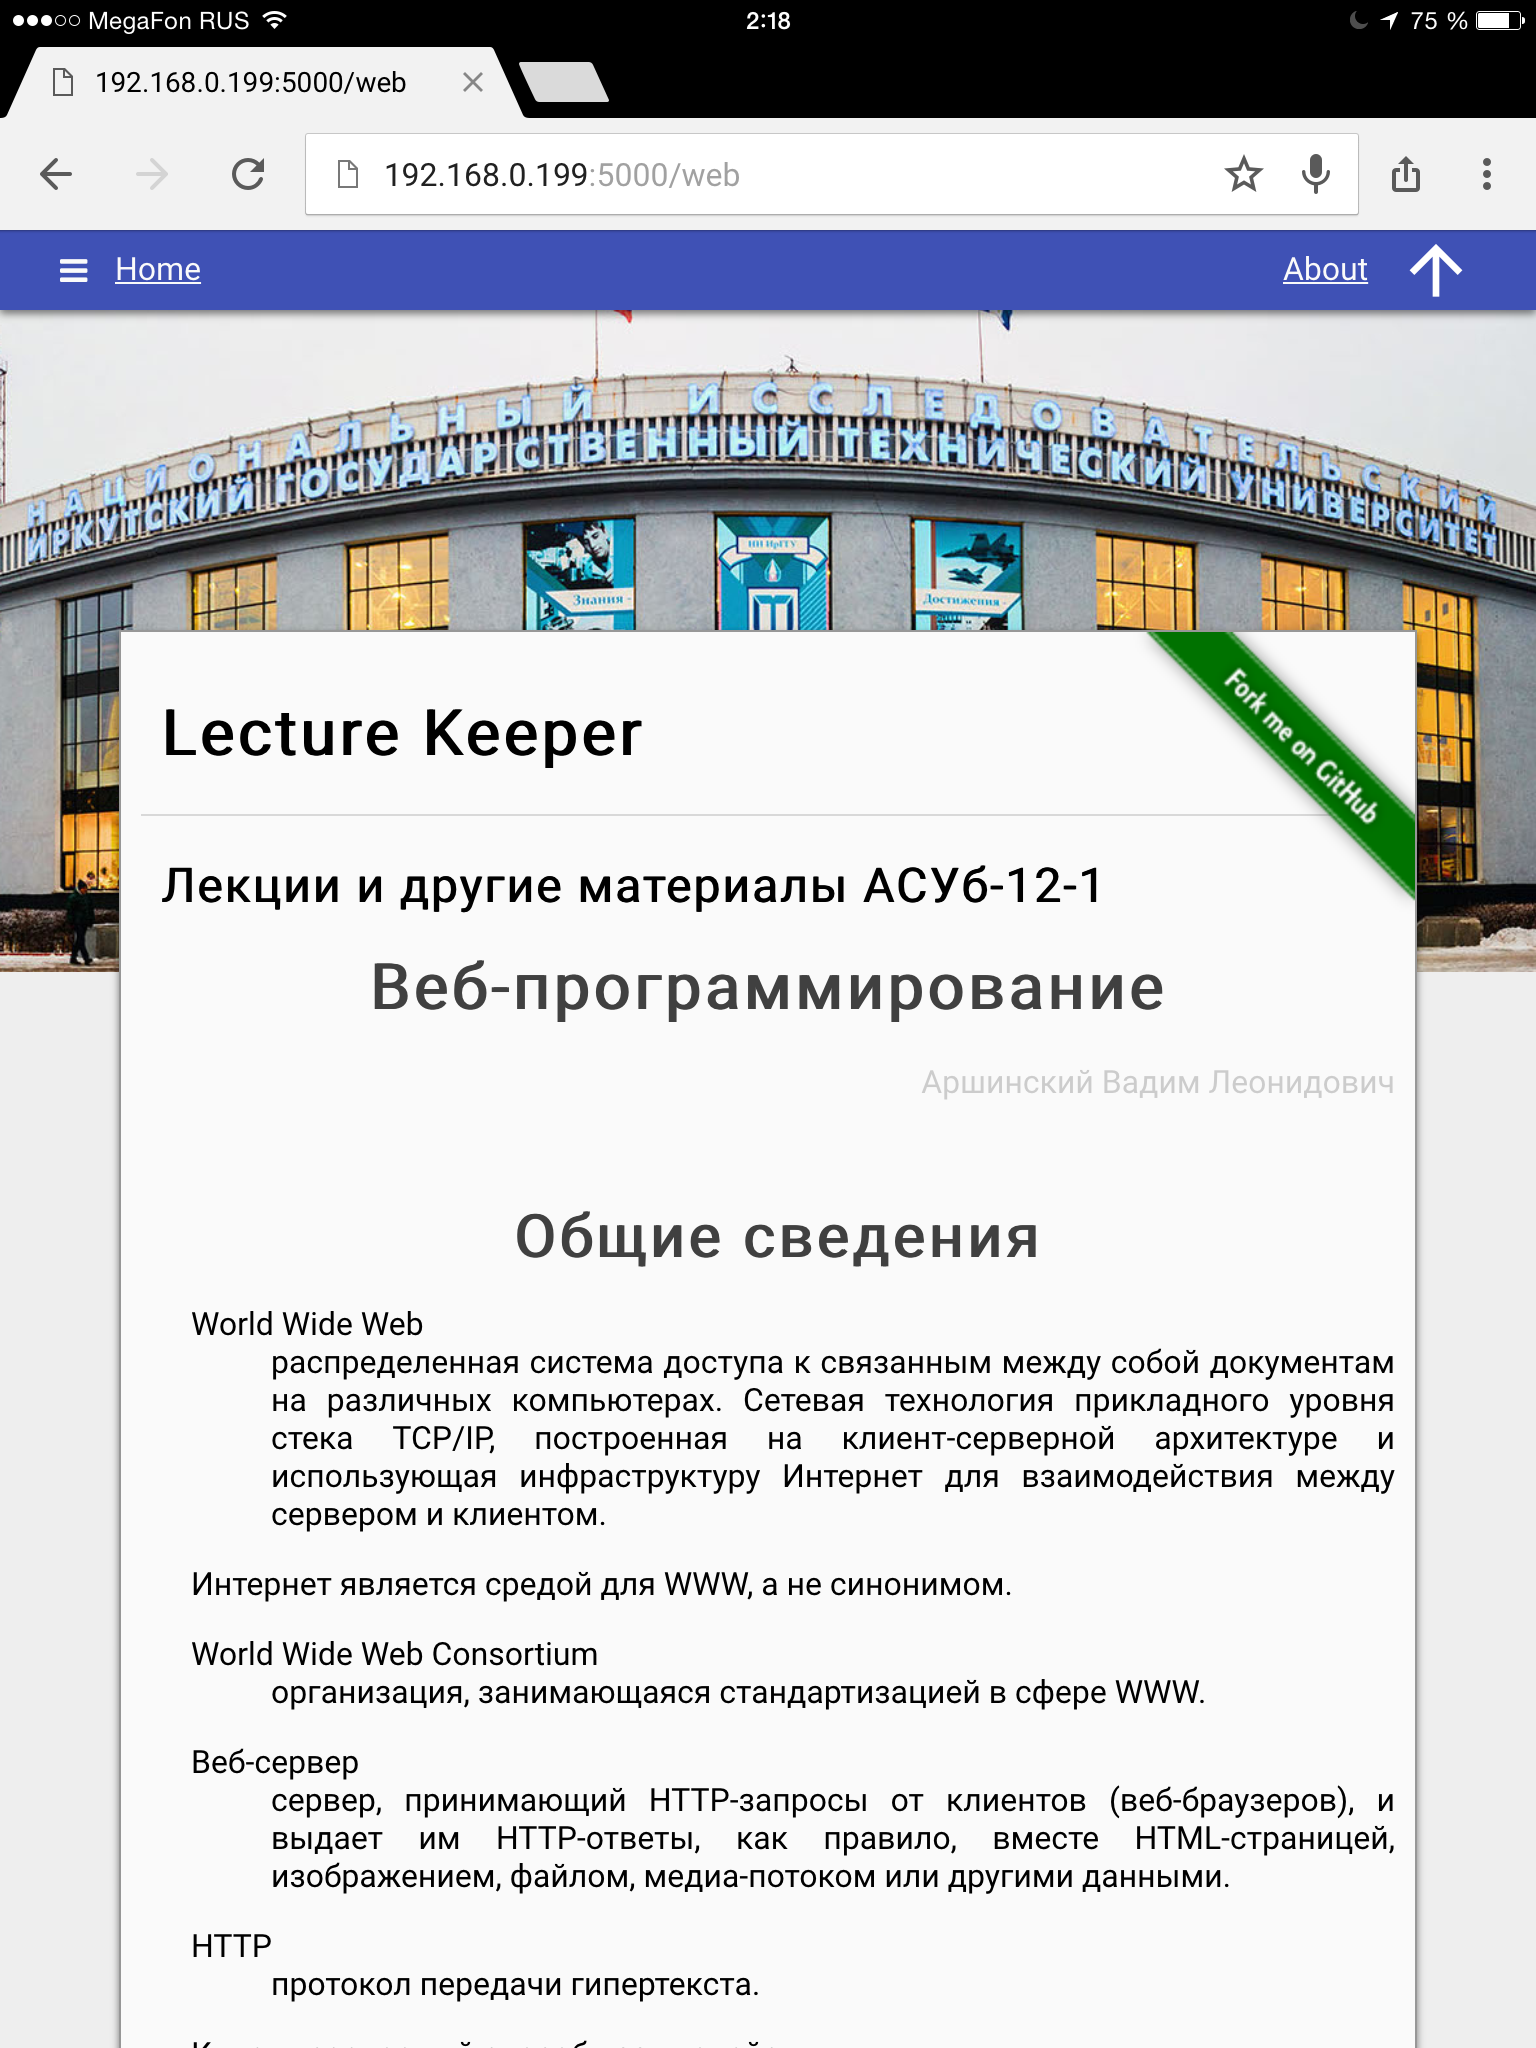
\includegraphics[width=\textwidth]{pics/screens/ipad_lec.png}
		\caption{iOS}
	\end{subfigure}
	\caption{Текст лекции}
\end{figure}

Как можно увидеть на рисунках, готовое приложение выглядит также, как и проектировалось на макетах. Небольшие различия объясняются итеративным подходом к разработке - некоторые изменения вносилились уже на этапе разработки.